\newpage
\subsubsection{UCS 5 - Gestione delle funzionalità di tracciamento dell'organizzazione}%kite level
\begin{figure}[h]
	\centering
    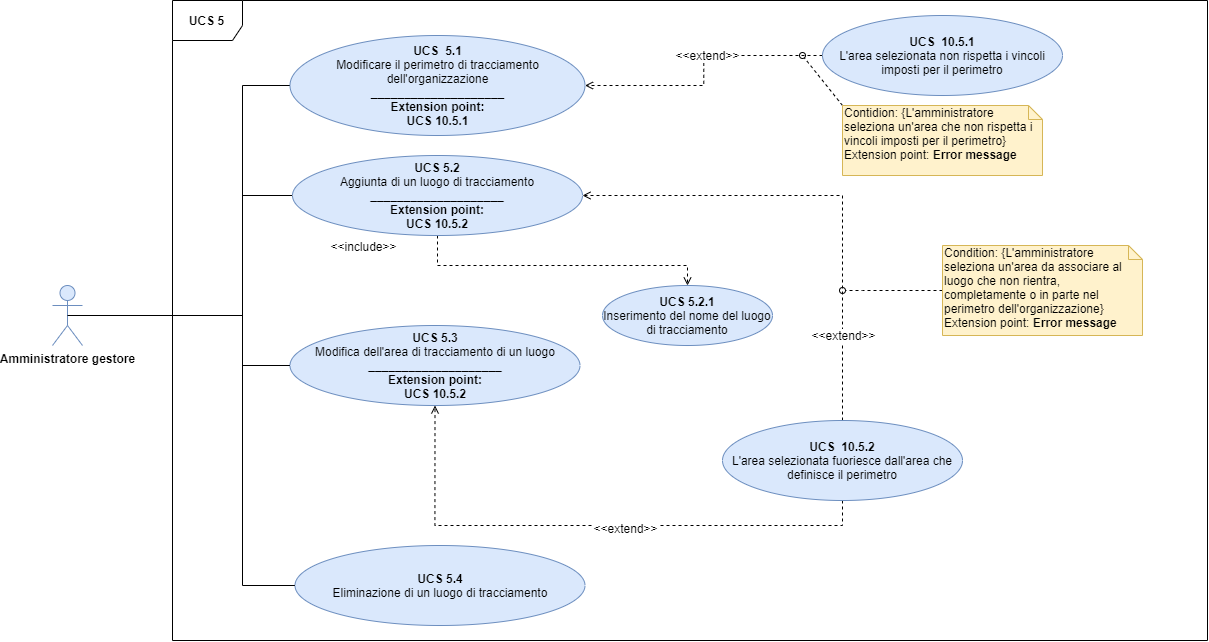
\includegraphics[scale=0.40]{Sezioni/UseCase/Immagini/UCS5.png}
    \caption{UCS 5 - Gestione delle funzionalità di \glo{tracciamento} dell'\glo{organizzazione}}
\end{figure}
\begin{itemize}
    \item \textbf{Attori primari:} Amministratore gestore
    \item \textbf{Precondizione:} L'amministratore si trova nella sezione di gestione dei parametri dell'\glo{organizzazione}.
    \item \textbf{Postcondizione:} L'amministratore ha gestito l'organizzazione riguardo al \glo{tracciamento} e ha salvato le modifiche, le quali sono state salvate nel sistema.
    \item \textbf{Scenario principale:} L'amministratore può:
    \begin{itemize}    
        \item Selezionare un nuovo \glo{perimetro} di \glo{tracciamento} dell'\glo{organizzazione} [UCS 5.1];
        \item Creare dei nuovi \glo{luoghi} di \glo{tracciamento} nell'\glo{organizzazione} [UCS 5.2];
        \item Modificare i \glo{luoghi} di \glo{tracciamento} dell'\glo{organizzazione} [UCS 5.3];
        \item Eliminare i \glo{luoghi} di \glo{tracciamento} dell'\glo{organizzazione} [UCS 5.4].
    \end{itemize}
\end{itemize}

\subsubsection{UCS 5.1 - Modificare il perimetro di tracciamento dell'organizzazione}%sea level
\begin{itemize}
    \item \textbf{Attori primari:} Amministratore gestore
    \item \textbf{Precondizione:} L'amministratore ha selezionato l’area geografica per il tracciamento dell'\glo{organizzazione}.
    \item \textbf{Postcondizione:} L'amministratore ha modificato con successo il \glo{perimetro} di \glo{tracciamento} dell'\glo{organizzazione}.
    \item \textbf{Scenario principale:} L'amministratore dovrà selezionare l'area geografica del \glo{perimetro} da tracciare.
     \item \textbf{Scenario alternativo:} L'amministratore ha selezionato un area che non rispetta i vincoli imposti. Verrà visualizzato un messaggio d'errore [UCS 10.5.1].
    \item \textbf{Flusso di eventi:}
    \begin{enumerate}%flusso di eventi
        \item L'amministratore seleziona la funzionalità di modifica del \glo{perimetro} di \glo{tracciamento} dell'\glo{organizzazione};
        \item L'amministratore seleziona un'area geografica da associare al \glo{perimetro} di \glo{tracciamento} dell'\glo{organizzazione} [UCS 5.5]. L'area selezionata deve rispettare i vincoli imposti.
    \end{enumerate}
    \item \textbf{Estensioni:}
    \begin{enumerate}
        \item UCS 10.5.1 - L'area selezionata non rispetta i vincoli imposti per il perimetro.
    \end{enumerate}
\end{itemize}

\subsubsection{UCS 5.2 - Aggiunta di un luogo di tracciamento}%sea level

\begin{figure}[h]
	\centering
    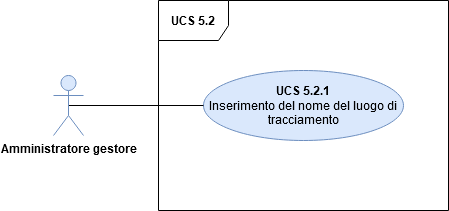
\includegraphics[scale=0.50]{Sezioni/UseCase/Immagini/UCS5.2.png}
    \caption{UCS 5.2 - Aggiunta di un luogo di tracciamento}
\end{figure}

\begin{itemize}
    \item \textbf{Attori primari:} Amministratore gestore
    \item \textbf{Precondizione:} L'amministratore ha selezionato l’area geografica per il tracciamento dell'\glo{organizzazione}.
    \item \textbf{Postcondizione:} L'amministratore ha aggiunto con successo un \glo{luogo} di tracciamento.
    \item \textbf{Scenario principale:} L'amministratore dovrà inserire i dati per il nuovo \glo{luogo} da tracciare e l'area geografica del luogo da tracciare.
    \item \textbf{Scenario alternativo:} L'amministratore ha selezionato un area che fuoriesce dall'area che definisce il \glo{perimetro}. Verrà visualizzato un messaggio d'errore [UCS 10.5.2].
    \item \textbf{Flusso di eventi:}
    \begin{enumerate}     
        \item L'amministratore seleziona la funzionalità per aggiungere un \glo{luogo} di tracciamento;
        \item Inserimento del nome del \glo{luogo} di \glo{tracciamento} [UCS 5.2.1];
        \item L'amministratore seleziona un'area geografica da associare al \glo{luogo} di tracciamento. L'area selezionata rispetta i vincoli imposti [UCS 5.5]; 
        \item L'amministratore seleziona la funzionalità per salvare le modifiche apportate.
    \end{enumerate}   
    \item \textbf{Estensioni:}
    \begin{enumerate}
        \item UCS 10.5.2 - L'area selezionata fuoriesce dall'area che definisce il perimetro.
    \end{enumerate}
\end{itemize}

\subsubsection{UCS 5.2.1 - Inserimento del nome del luogo di tracciamento}%sea level
\begin{itemize}
    \item \textbf{Attori primari:} Amministratore gestore
    \item \textbf{Precondizione:} L'amministratore si trova nella sezione di modifica dei \glo{parametri dell'organizzazione}.
    \item \textbf{Postcondizione:} L'amministratore ha inserito un nome valido per il \glo{luogo} di tracciamento.
    \item \textbf{Scenario principale:} Inserimento del nome del luogo di tracciamento.
\end{itemize}

\subsubsection{UCS 5.3 - Modifica dell'area di tracciamento di un luogo}%sea level
\begin{itemize}
    \item \textbf{Attori primari:} Amministratore gestore
    \item \textbf{Precondizione:} L'amministratore ha selezionato l’area geografica per il tracciamento dell'\glo{organizzazione}.
    \item \textbf{Postcondizione:} L'amministratore ha modificato con successo l'area di \glo{tracciamento} del \glo{luogo}.
    \item \textbf{Scenario principale:} L'amministratore dovrà selezionare una nuova area per il \glo{tracciamento} del \glo{luogo} scelto.
    \item \textbf{Scenario alternativo:} L'amministratore ha selezionato un area che fuoriesce dall'area che definisce il \glo{perimetro}. Verrà visualizzato un messaggio d'errore [UCS 10.5.2].
    \item \textbf{Flusso di eventi:}
    \begin{enumerate}%flusso di eventi
        \item L'amministratore seleziona la funzionalità per modificare l'area di \glo{tracciamento} di un \glo{luogo};
        \item L'amministratore seleziona il \glo{luogo} da modificare;
        \item L'amministratore seleziona un'area geografica da associare al \glo{luogo} di \glo{tracciamento} [UCS 5.5];
        \item L'amministratore seleziona la funzionalità per salvare le modifiche apportate.
    \end{enumerate}
    \item \textbf{Estensioni:}
    \begin{enumerate}
        \item UCS 10.5.2 - L'area selezionata fuoriesce dall'area che definisce il perimetro.
    \end{enumerate}
\end{itemize}

\subsubsection{UCS 5.4 - Eliminazione di un luogo di tracciamento}%sea level
\begin{itemize}
    \item \textbf{Attori primari:} Amministratore gestore
    \item \textbf{Precondizione:} L'amministratore si trova nella sezione di modifica dei parametri dell'\glo{organizzazione}.
    \item \textbf{Postcondizione:} L'amministratore ha eliminato con successo il \glo{luogo} di \glo{tracciamento} desiderato.
    \item \textbf{Scenario principale:} L'amministratore elimina un \glo{luogo} di \glo{tracciamento} definito all'interno dell'\glo{organizzazione}.
    \item \textbf{Flusso di eventi:}
    \begin{enumerate}%flusso di eventi
        \item L'amministratore seleziona la funzionalità per eliminare un \glo{luogo} dell'\glo{organizzazione};
        \item L'amministratore seleziona il \glo{luogo} da eliminare;
        \item L'amministratore seleziona la funzionalità di conferma per rendere definitiva l'eliminazione del \glo{luogo} di tracciamento.
    \end{enumerate}
\end{itemize}

\subsubsection{UCS 5.5 - Selezione dell'area geografica per il tracciamento}%sea level

\begin{figure}[h]
	\centering
    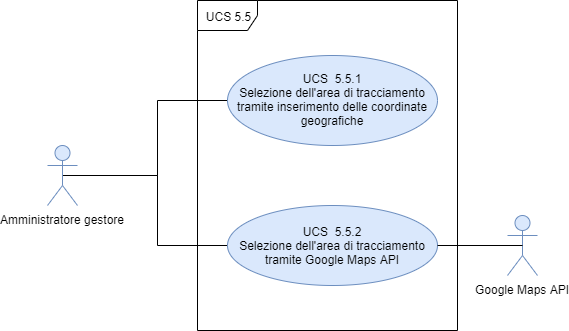
\includegraphics[scale=0.50]{Sezioni/UseCase/Immagini/UCS5.5.png}
    \caption{UCS 5.5 - Selezione dell'area geografica per il tracciamento}
\end{figure}

\begin{itemize}
\item \textbf{Attori primari:} Amministratore gestore
\item \textbf{Precondizione:} L'amministratore si trova nella sezione di modifica dei \glo{parametri dell'organizzazione}.
\item \textbf{Postcondizione:} L'amministratore ha selezionato un'area per il \glo{tracciamento}.
\item \textbf{Scenario principale:} L'amministratore deve selezionare un'area geografica per il \glo{tracciamento} del \glo{luogo} scelto.
\item \textbf{Scenario alternativo:} L'amministratore vuole uscire dalla funzionalità di selezione dell'area geografica per il \glo{tracciamento} [UCS 10.5.3].
\item \textbf{Flusso di eventi:}
\begin{enumerate}
    \item L'amministratore seleziona la funzionalità di selezione dell'area;
    \item Sceglie dunque se il fine dell'area da tracciare è per un \glo{luogo} dell'\glo{organizzazione} oppure è per il \glo{perimetro} di tracciamento;
    \item L'amministratore può scegliere se selezionare l'area inserendo le coordinate geografiche [UCS 5.5.1] oppure tramite Google Maps API [UCS 5.5.2].
\end{enumerate}
\item \textbf{Estensioni:}
    \begin{enumerate}
        \item UCS 10.5.3 - Annullamento della selezione dell'area geografica per il tracciamento.
    \end{enumerate}
\end{itemize}

\subsubsection{UCS 5.5.1 - Selezione dell'area di tracciamento tramite inserimento delle coordinate geografiche}%fish level
\begin{itemize}
\item \textbf{Attori primari:} Amministratore gestore
\item \textbf{Precondizione:} L'amministratore si trova nella sezione di modifica dei \glo{parametri dell'organizzazione}, in particolare nella sezione di selezione.
\item \textbf{Postcondizione:} L'amministratore ha inserito le coordinate geografiche che delimitano un'area per il \glo{tracciamento}.
\item \textbf{Scenario principale:} Selezione dell'area di tracciamento tramite inserimento delle coordinate geografiche.
\item \textbf{Flusso di eventi:}
\begin{enumerate}
    \item L'amministratore inserisce un certo numero di coordinate per i rispettivi vertici dell'area di \glo{tracciamento};
\end{enumerate}
\item \textbf{Generalizzazione:}
	\begin{enumerate}
        \item UCS 5.5 - Selezione dell'area geografica per il tracciamento;
    \end{enumerate}
\end{itemize}

\subsubsection{UCS 5.5.2 - Selezione dell'area di tracciamento tramite Google Maps API}%fish level
\begin{itemize}
\item \textbf{Attori primari:} Amministratore gestore
\item \textbf{Attori secondari:} Google Maps API
\item \textbf{Precondizione:} L'amministratore si trova nella sezione di modifica dei \glo{parametri dell'organizzazione}, in particolare nella sezione di selezione.
\item \textbf{Postcondizione:} L'amministratore ha selezionato un'area per il \glo{tracciamento} usufruendo dell'interfaccia di Google Maps API.
\item \textbf{Scenario principale:} Selezione dell'area di tracciamento tramite Google Maps API.
\item \textbf{Flusso di eventi:}
\begin{enumerate}
    \item L'amministratore interagisce con Google Maps API per selezionare l'area di \glo{tracciamento}.
\end{enumerate}
\item \textbf{Generalizzazione:}
	\begin{enumerate}
        \item UCS 5.5 - Selezione dell'area geografica per il tracciamento;
    \end{enumerate}
\end{itemize}

